\documentclass{classrep}
\usepackage[utf8]{inputenc}
\usepackage{color}
\usepackage{amsmath}
\usepackage[T1]{fontenc}
\usepackage{graphicx}
\usepackage[section]{placeins}

\studycycle{Informatyka, studia niestacjonarne, I st.}
\coursesemester{VI}

\coursename{Komputerowe systemy rozpoznawania}
\courseyear{2019}

\courseteacher{dr hab. inż. Adam Niewiadomski}
\coursegroup{Niedziela, 12:00}

\author{
  \studentinfo{Konrad Jachimstal}{211807} \and
  \studentinfo{ Patryk Janicki}{211951}
}

\title{Zadanie 1: Ekstrakcja cech, miary podobieństwa, klasyfikacja}

\begin{document}
\maketitle

\section{Cel}
{Celem zadania jest zbadanie wpływu ekstrakcji cech oraz wykorzystanych miar podobieństwa w procesie klasyfikacji tekstu. 
Klasyfikacja tekstów ma zostać zrealizowania z wykorzystaniem algorytmu najbliższych sąsiadów (KNN).}

\section{Wprowadzenie}
Do wykonania tego zadania niezbędne będzie skorzystanie z uczenia maszynowego.
Klasyfikacja tekstów, która odbywa się za pomocą algorytmu KNN. Polega ona na przypisaniu tekstu do odpowiedniej
kategorii. Odbywa się to na podstawie watrości poszczególnych wyekstrachowanych cech, które posiada każdy z tekstów.\\
Do ekstrakcji wykorzystywany jest znormalizowany zbiór słów badanego tekstu, oznaczony przez T. Normalizacja ma na
celu wyeliminowanie niepożądanych słów oraz sprowadzenie odmian słów o tym samym znaczeniu do jednego (określenie rdzenia słowa).
\clearpage

\subsection{Wykorzystane cechy}
\subsubsection{Występowanie słowa kluczowego}
Na podstawie dostarczonego słowa kluczowego określamy czy to słowo występuje w dokumencie (reprezentacja binarna).
Przy użyciu tej cechy nie bierzemy pod uwagę liczności występowania tego słowa kluczowego. Cecha przyjmuje wartości $\{0; 1\}$.
\begin{equation}
    F=\left\{\begin{matrix}
                 1, & kiedy\ w = t_{i}\\
                 0, & w\ przeciwnym\ przypadku
    \end{matrix}\right.
\end{equation}
gdzie:\\
\begin{description}
    \item $w$ - dane słowo kluczowe;
    \item $t_{1}$ - kolejne słowa występujące w tekście;
\end{description}

\subsubsection{Liczba wystąpień słowa kluczowego}
Na podstawie dostarczonego słowa kluczowego określamy liczbę wystąpień tego słowa w dokumencie. Wykorzystanie tej cechy dla listy
słów kluczowych pozwala na stwierdzenie  jak licznie występuje każde słowo kluczowe w dokumencie. Chcemy sprawdzić,
czy określenie liczności słów kluczowych ma istotny wpływ na klasyfikację dokumentu.
\begin{equation}
    F=\sum_{i=0}^{n} S(w)
\end{equation}
gdzie:
\begin{equation} \label{eq:1}
    S(w)=\left\{\begin{matrix}
                    1, & kiedy\ w = t_{i}\\
                    0, & w\ przeciwnym\ przypadku
    \end{matrix}\right.
\end{equation}\\ oraz:
\begin{description}
    \item $t_{i}$ - kolejne słowa występujące w tekście;
    \item $n$ - liczba słów kluczowych;
\end{description}

\subsubsection{Suma wystąpień słów kluczowych}
Wystąpienie w dokumencie wszystkich słów kluczowych z listy ma istotny wpływ na to w jakim stopniu dany tekst
przynależy do danej etykiety. Cecha to liczba całkowita przyjmująca wartości z przedziału $<0; n>$ gdzie $n$ liczba słów w tekście.
\begin{equation}
    F=S_{1} + ... + S_{n}
\end{equation}
gdzie:\\
\begin{description}
    \item $S$ - liczba wystąpień słowa kluczowego;
\end{description}

\clearpage
\subsubsection{Gęstość występowania słów kluczowych}
Wyliczenie gęstości słów klyczowych pozwala na sprawdzenie czy cały dokument stanowi na dany temat czy jest to
jedynie wzmianka. Cecha to liczba przyjmująca wartości z zakresu $<0; 1>$.
    \begin{equation}
      F=\frac{S}{L}
    \end{equation}
gdzie:\\
\begin{description}
    \item $S$ - suma wystąpień słów kluczowych;
    \item $L$ - liczba wszystkich słów w tekście;
\end{description}

\subsubsection{Odległość słowa kluczowego od początku tekstu}
Odległość słowa kluczowego od początku tekstu wyrażona za pomocą sumy liczby wyrazów poprzedzających
dane słowo kluczowe.
Cecha przyjmuje wartości liczbowe z zakresu $<0; n>$, gdzie $n$ - liczba wyrazów poprzedzających słowo kluczowe.
\begin{equation}
    F=\sum_{0}^{n}1
\end{equation}
gdzie:\\
\begin{description}
    \item $n$ - liczba wyrazów poprzedzających dane słowo kluczowe;
\end{description}


\subsubsection{Średnia odległość słów kluczowych od początku tekstu}
Średnia odległość słów kluczowych wyrażona jako iloraz sumy odległości słów kluczowych od początku tekstu i liczby
słów kluczowych w tekście. Cecha to suma wartości liczbowych odzwierciedlających odległość danego słowa kluczowego
od początku tekstu, gdzie pojedyncze słowo odpowiada odległości równej jeden. Cecha przyjmuje wartości $<0; n>$ gdzie n
jest maksymalną średnią z sumy odległości słów kluczowych od początku tekstu.
\begin{equation}
    F=\frac{S_{1} + ... + S_{n}}{L}
\end{equation}
gdzie:\\
\begin{description}
    \item $S$ - odległość słowa kluczowego od początku tekstu;
    \item $L$ -  liczba słów kluczowych w tekście;
\end{description}

\subsubsection{Pierwsze słowo kluczowe}
Pierwsze słowo kluczowe przyjmuje wartość pierwszego napotkanego słowa kluczowego w tekście. Cecha przyjmuje wartość
tekstową odpowiadającą pierwszemu napotkanemu słowu kluczowemu.
\begin{equation}
    F= h(i)=\left\{\begin{matrix}
       w, & w = t_{i}
    \end{matrix}\right.
\end{equation}
gdzie:\\
\begin{description}
    \item $w$ - dane słowo kluczowe;
    \item $t_{i}$ - kolejne słowa występujące w tekście;
\end{description}

\subsubsection{Najczęściej występujące słowo kluczowe}
Najczęściej występujące słowo kluczowe wyrażone jako tekst odpowiadający największej liczbie wystąpień danego
słowa kluczowego w tekście. Cecha przyjmuje wartość tekstową odpowiadającą najczęściej występującemu słowu kluczowemu.
\begin{equation}
    F= w_{max_{i}(h(w_{i}), h(w_{i}))}
\end{equation}
gdzie:
\begin{equation}
    h(w)=\sum_{i=0}^{n} S(w)
\end{equation}
\begin{description}
    \item $S(w)$ - według wzoru (\ref{eq:1});
    \item $w$ - dane słowo kluczowe;
    \item $t_{i}$ - kolejne słowa występujące w tekście;
\end{description}

\subsubsection{Liczba wszystkich słów}
Określenie liczby wszystkich słów występujących w tekście. 
Cecha przyjmuje wartość $n$ równą liczbie słów w tekście.
\begin{equation}
    F=|S|
\end{equation}
gdzie:\\
\begin{description}
    \item $S$ - to zbiór słów występujących w tekście;
\end{description}

%\subsubsection{Rozproszenie słów kluczowych}
%Rozproszenie słów kluczowych wyrażone jako iloraz sumy odległości pomiędzy słowami kluczowymi i iloczyn liczby
%wszystkich słów w tekście oraz liczby słów kluczowych w tekście.
%
%Możemy podjąć próbę i założyć, że większe nagromadzenie słów kluczowych na przestrzeni całego tekstu pozwala
%stwierdzić, czy określone słowa kluczowe mają powiązanie z tematem tekstu, a nie stanowią wzmianki czy wstępu do
%tekstu. Ekstrakcja ma pozwolić na określenie rozrzutu słów kluczowych w tekście. Cecha jest określona na podstawie
%sumy odległości pomiędzy słowami kluczowymi z uwzględnieniem gęstości ich występowania. Przyjmuje wartości $[0, \infty]$.
%\begin{equation}
%    F=\frac{E_{d}}{N*N_{k}}
%\end{equation}
%gdzie:\\
%\begin{description}
%    \item $E_{d}$ - suma odległości pomiędzy słowami kluczowymi;
%    \item $N$ - liczba wszystkich słów w tekście;
%    \item $N_{k}$ - liczba słów kluczowych w tekście;
%\end{description}

%\subsubsection{Występowanie określonych podciągów}
%\dots
\subsection{Określanie istotności słów}
Podczas analizy tekstu można zauważyć, że niektóre słowa są bardziej lub mniej istotne. W związku z tym zależy nam
na eliminacji słów nieznaczących i wyodrębnieniu słów istotnych w kontekście dokumentu. Istotność słów możemy określić
na podstawie następujących algorytmów opisanych poniżej.


\subsubsection{Częstość słów (ang. Term Frequency)}
Liczba wystąpień słowa w dokumencie w stosunku do wszystkich słów pozwala nam na określenie częstotliwości występowania
określonego słowa. Zakładamy, że słowo, które występuje stosunkowo rzadko w dokumencie jest wysoce istotne. Zależność tą
można określić za pomocą wzoru:
\begin{equation}
    F=\frac{K}{W}
\end{equation}
gdzie:\\
\begin{description}
    \item $K$ - liczba wystąpień danego słowa kluczowego w dokumencie;
    \item $W$ - liczba wszystkich słów w dokumencie;
\end{description}

\subsubsection{IDF (ang. inverse document frequency)}
Możemy określić w ilu dokumentach występuje dane słowo. Jeśli słowo występuje w małej liczbie dokumentów lub tylko w
jednym, można stwierdzić, że to słowo jest ściśle powiązane z treścią tych dokumentów. Zależność tą można określić za
pomocą wzoru:
\begin{equation}
    F=log \frac{W}{D}
\end{equation}
gdzie:\\
\begin{description}
    \item $W$ - liczba wszystkich dokumentów;
    \item $D$ - liczba dokumentów w których wystąpiło słowo kluczowe;
\end{description}

\subsubsection{TF-IDF}
Jest to połączenie częstości słów występujących w dokumencie zestawione z stosunkiem wytępowania tego słowa we wszystkich
dokumentach. Połączenie tych cech pozwala na uzależnienie istotności słowa nie tylko od dokumentu w którym występuje,
ale również od występowania w całym zbiorze dokumentów. Zależność tą można określić za pomocą wzoru:
\begin{equation}
    F={TF}\cdot{IDF}
\end{equation}
gdzie:\\
\begin{description}
    \item $TF$ - częstość słów w danym dokumencie;
    \item $IDF$ - częstość występowania na tle innych dokuemntów;
\end{description}

\subsubsection{Generowanie stop listy}
Tworzenie stop listy opieramy na algorytmie IDF. Słowo które ma najmniejszą wartość IDF występuje najczęściej. Czyli jest
nieistotne. Dodajemy do stoplisty jeśli dana wartość będzie poniżej określonego progu.

\subsubsection{Nauka słów kluczowych}
Do nauki słów kluczowych wykorzystujemy algorytm TF-IDF, za pomocą którego określamy istotność
danego słowa. Kiedy dla danego słowa wartość ta jest większą od założonej, uznajemy to słowo za istotne tym samym dopisując je do
listy słów kluczowych. Słowa kluczowe mogą zostać również określone odgórnie.

\subsection{Metryki - miara odległości}
Wykorzystane metryki służa do określenia odległości pomiędzy elementami tego samego zbioru w naszym przypadku tym
zbiorem będzie zbiór artykułów. Do obliczenia odległości pomiędzy dwoma artykułami na potrzeby algorytmu KNN zostały
wykorzystane metryki opisane poniżej.

\subsubsection{Metryka Euklidesowa}
Odległość Euklidesowa jest to odległość między dwoma wektorami określona jako pierwiastek kwadratowy sumy różnic między
wartościami podniesionymi do kwadratu, wyrażona wzorem:
\begin{equation}
    d(x,y)=\sqrt{\sum_{i=1}^{n}((x_{i}-y_{i})^{2})}
\end{equation}
gdzie:\\
\begin{description}
    \item $d$ - miara odległości;
    \item $x$, $y$ - wartości cech;
\end{description}

\subsubsection{Metryka Czebyszewa}
Odległość Czebyszewa jest to różnica pomiędzy znormalizowanymi cechami wartości obiektów, określona wzorem:
\begin{equation}
    d(x,y)=max_{i}|x_{i}-y_{i}|
\end{equation}
gdzie:\\
\begin{description}
    \item $d$ - miara odległości;
    \item $x$, $y$ - wartości cech obiektów;
\end{description}

\subsubsection{Metryka Manhattana}
Metryka Manhattana jest metryką podobną do metryki euklidesowej z tą różnicą, że odległość wyliczana jest
z bezwzględnych różnic pomiędzy wektorami. Odległość tę wyraża się wzorem:
\begin{equation}
    d(x,y)=\sum_{i=1}^{n} |x_{i}-y_{i}|
\end{equation}
gdzie:\\
\begin{description}
    \item $d$ - miara odległości;
    \item $x$, $y$ - wartości cech obiektów;
\end{description}

\subsection{Miary podobieństwa tekstów}
Miara podobieństwa tesktów to miara mówiąca o tym w jakim stopniu dany tekst $A$ jest podobny do tekstu $B$.

\subsubsection{Metoda n-gramów}
Metoda n-gramów określa w jakim stopniu łańcuch znaków $x$ jest podobny do łańcucha znaków $y$, na podstawie podciągów.
\begin{equation}
    sim_{n}(x,y)=\frac{1}{N-n+1}\sum_{i=1}^{N-n+1}h(i)
\end{equation}
gdzie:\\
\begin{description}
    \item $h(i)$ - przyjmuje 1 jeżeli dany podciąg występuje w łancuchu znaków $y$, w przeciwnym wypadku przyjmuje wartość 0;
    \item $N$ - liczba liter w słowie;
    \item $n$ - długość n-grama;
    \item $N-n+1$ - ilość n-elementowych podciągów w łańcuchu znaków;
\end{description}

\subsubsection{Uogólniona miara n-gramów}
Uogólniona miara n-gramów sprawdza podobieństwo słów w oparciu o podciągi o określonej długości. Wyrażona jest wzorem:

\begin{equation}
    u_{N}(x, y)=\frac{2}{N^{2}+N}\sum_{i=1}^{N(x)}\sum_{j=1}^{N(x-i+1)}h(i,j)
\end{equation}
gdzie:\\
\begin{description}
    \item $h(i,j)$ przyjmuje wartość 1 jeżeli dany podciąg ze słowa $x$ znajduje się w słowie $y$;
    \item $N(x),N(y)$ - ilość liter w słowach $x, y$, $N=max{N(x),N(y)}$;
    \item $\frac{N^{2}+N}{2}$ - ilość możliwych podciągów 1-elementowych do N-elementowych w słowie o długości $N$;
\end{description}

\subsubsection{Algorytm KMP (Knutha-Morrisa-Pratta)}
Algorytm KMP wyszukuje podany wzorzec $x$ w tekście $y$, jeżeli podany wzorzec zostaje znaleziony zwracana jest jego
pozycja w tekście. Wyrażony jest wzorem:
\begin{equation}

\end{equation}
gdzie:\\
\begin{description}
    \item
    \item
    \item
\end{description}

\subsection{Określanie poprawności klasyfikacji}
Poprawność sklasyfikowanych danych określa w jakim stopniu dokumenty zostały poprawnie przyporządkowane etykietom.
Wartość poprawności będzie oscylować w przedziale $<0;1>$. Kiedy wartość będzie będzie zbliżać się do jedynki będzie
to oznaczać, że większość dokumentów została sklasyfikowana poprawnie.

\begin{equation}
    F=\frac{P}{W}
\end{equation}
gdzie:\\
\begin{description}
    \item $P$ - liczba poprawnie sklasyfikowanych dokumentów
    \item $W$ - liczba wszystkich klasyfikacji
\end{description}



\newline \newline
{\color{blue}
We wprowadzeniu należy zaprezentować całą teorię potrzebną do realizacji
zadania (przy czym należy tu ograniczyć się wyłącznie do tego, co było
wykorzystane) tak aby osoba, która nigdy wcześniej nie zetknęła się z tą
tematyką, potrafiła zrozumieć dalszy opis. Część ta powinna wprowadzać
wszystkie wykorzystywane wzory, oznaczenia itp., do których należy się
odwoływać w dalszej części niniejszgo sprawozdania. Zamieszczony tu własny
opis teorii (a nie skopiowany!) należy poprzeć odwołaniami bibliograficznymi
do literatury zamieszczonej na końcu. }

\section{Opis implementacji}
Projekt został zaimplementowany w języku Java. W celu łatwiejszej nawigacji został podzielony na poszczególne pakiety:
\begin{itemize}
    \item data\_models
    \item features
    \item helpers
    \item metrics
    \item similarity
    \item utils
    \item gui
\end{itemize}
Z powyższych pakietów możemy wyszczególnić najważniejsze klasy ze względu na tematykę projektu. Podstawowym pakietem
jest pakiet "data\_model", w którym to wczytywane są z pliku artykuły a następnie dzielone na poszczególne klasy "Article".
Klasa "Extraction" zawiera w sobie wszystkie wykorzystane w programie cechy z podziałem każdej cechy jako jedną metodę.
Daje to możliwość skorzystania jedynie z cech, które nas interesują. W pakiecie "metrics" zostały zaimplementowane metody
liczenia odległości pomiędzy wektorami cech na podstawie interfejsu "IMetric", w którym to zadeklarowana została
metoda "compare" służąca do porównywania wektorów cech. Pakiet "similarity" odpowiada za liczenie odległości w
przpadkach kiedy cecha jest słowem. Klasa "TermFrequency" wykorzystywana jest podczas generowania słów kluczowych oraz stop listy.
Wszystkie klasy wykorzystane zostają w klasie "Classification", dokounuje się tam wszystkich operacji począwszy od podziału
tekstów na dwa zbiory po klasyfikację tekstu do odpowiedniej etykiety.

\begin{figure}[h!]
    \centering
    \makebox[\textwidth][c]{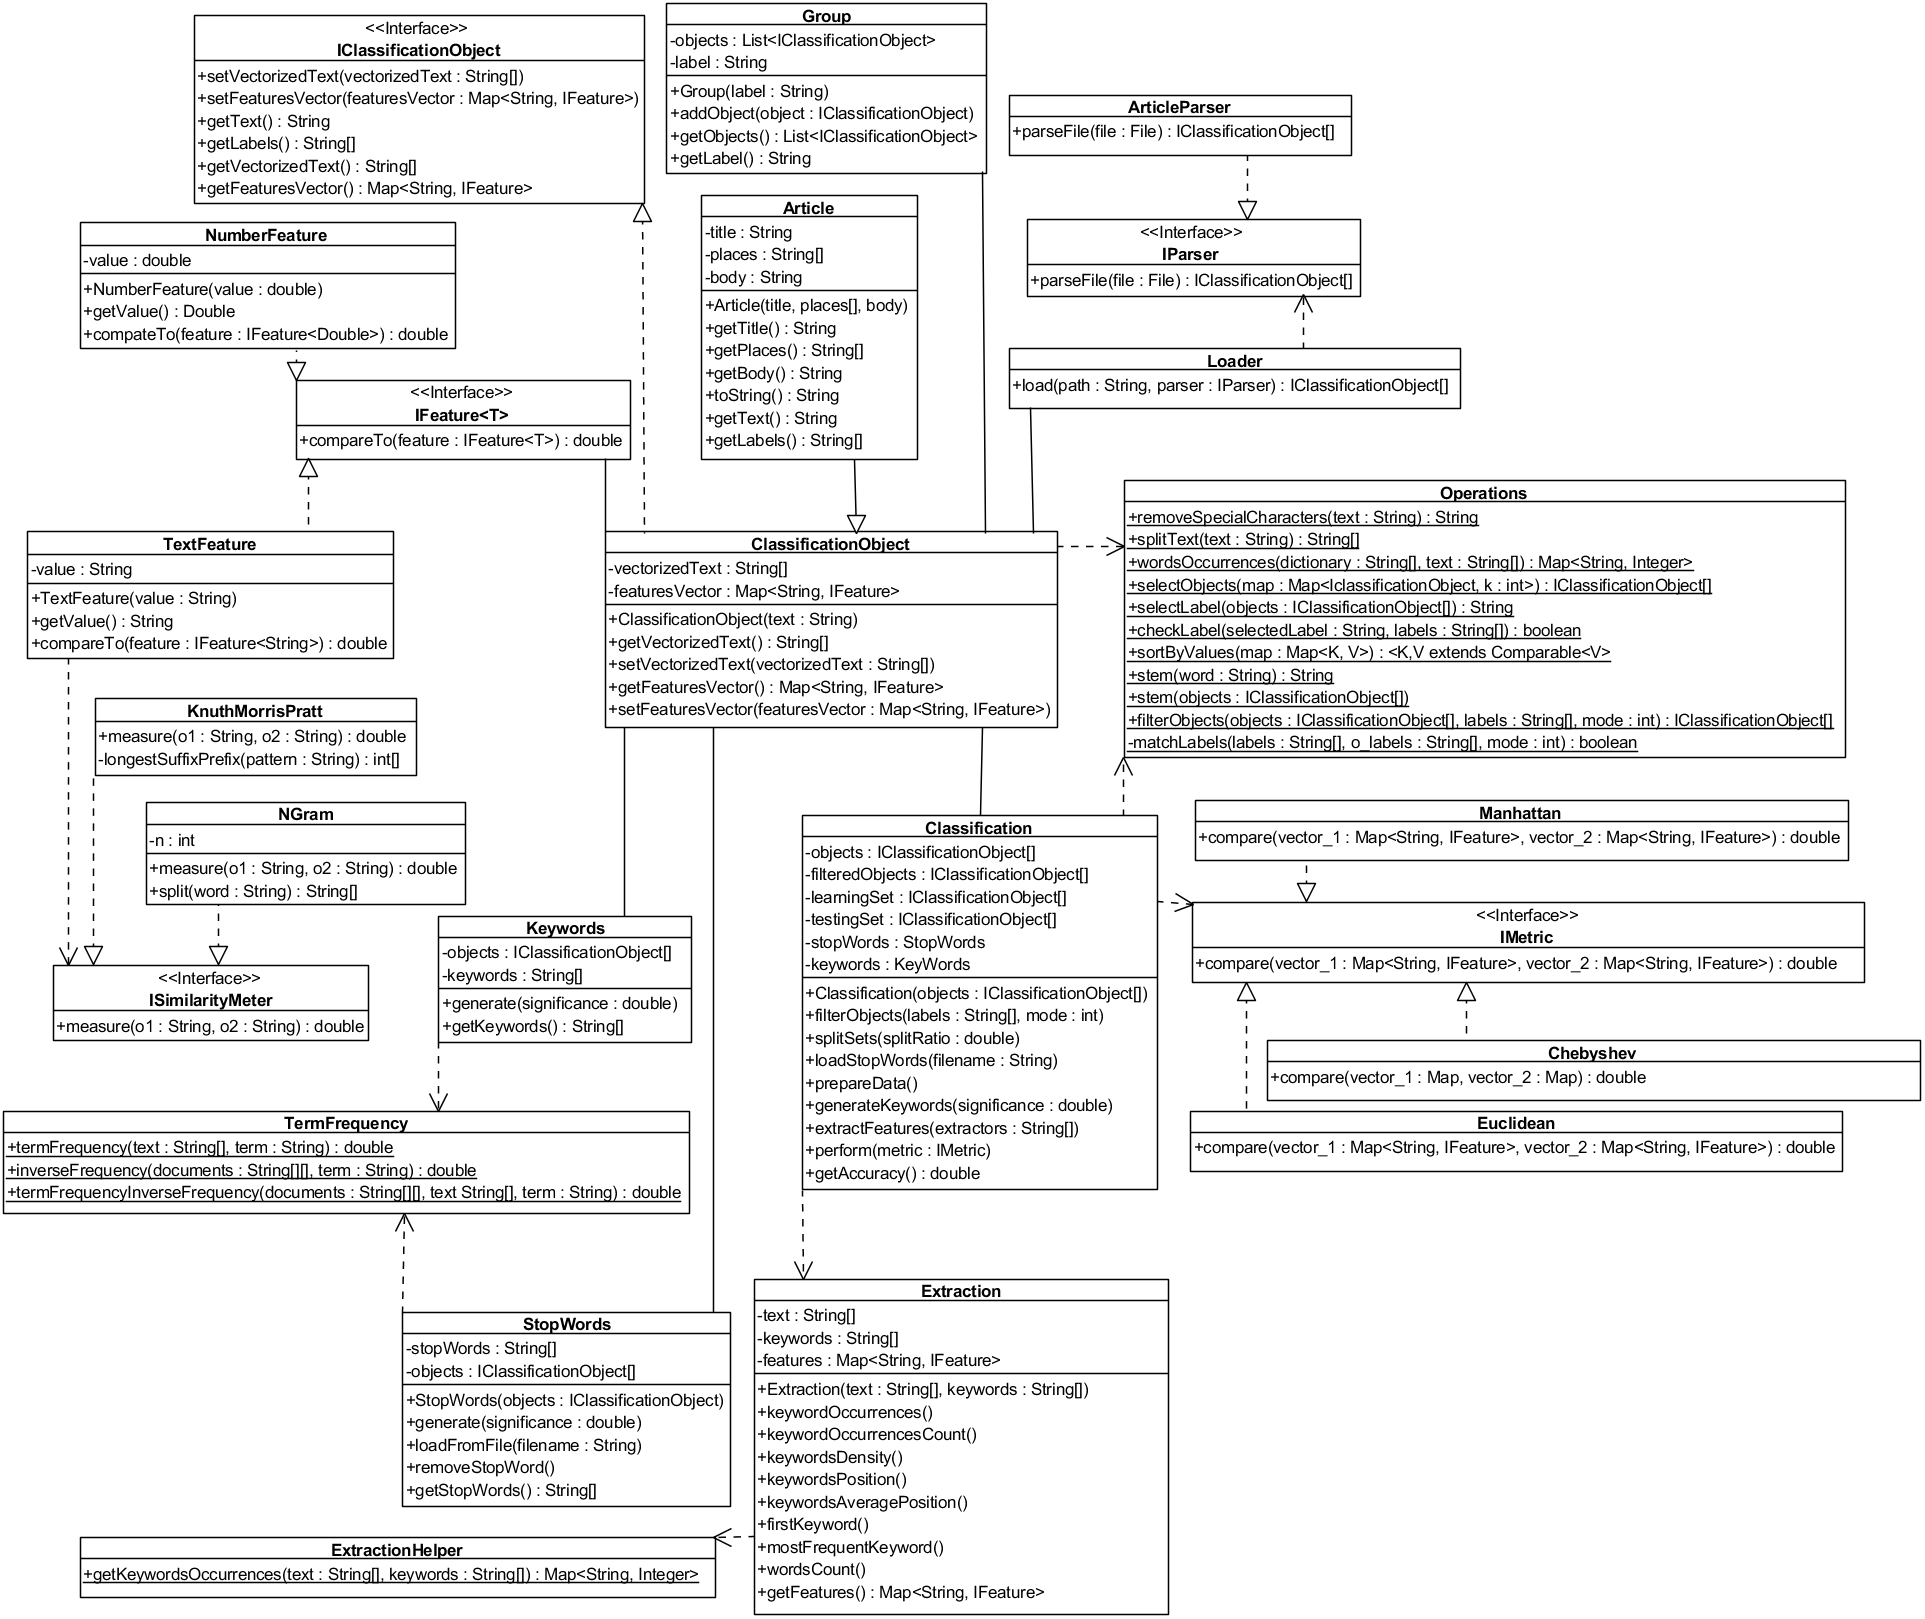
\includegraphics[width=18cm\textwidth]{uml.png}}%
    \caption{Diagram klas}
    \label{fig:uml}
\end{figure}



{\color{blue}
Należy tu zamieścić krótki i zwięzły opis zaprojektowanych klas oraz powiązań
między nimi. Powinien się tu również znaleźć diagram UML  (diagram klas)
prezentujący najistotniejsze elementy stworzonej aplikacji. Należy także
podać, w jakim języku programowania została stworzona aplikacja. }

\section{Materiały i metody}

{\color{blue}
W tym miejscu należy opisać, jak przeprowadzone zostały wszystkie badania,
których wyniki i dyskusja zamieszczane są w dalszych sekcjach. Opis ten
powinien być na tyle dokładny, aby osoba czytająca go potrafiła wszystkie
przeprowadzone badania samodzielnie powtórzyć w celu zweryfikowania ich
poprawności (a zatem m.in. należy zamieścić tu opis architektury sieci,
wartości współczynników użytych w kolejnych eksperymentach, sposób
inicjalizacji wag, metodę uczenia itp. oraz informacje o danych, na których
prowadzone były badania). Przy opisie należy odwoływać się i stosować do
opisanych w sekcji drugiej wzorów i oznaczeń, a także w jasny sposób opisać
cel konkretnego testu. Najlepiej byłoby wyraźnie wyszczególnić (ponumerować)
poszczególne eksperymenty tak, aby łatwo było się do nich odwoływać dalej.}

\section{Wyniki}
{\color{blue}
W tej sekcji należy zaprezentować, dla każdego przeprowadzonego eksperymentu,
kompletny zestaw wyników w postaci tabel, wykresów itp. Powinny być one tak
ponazywane, aby było wiadomo, do czego się odnoszą. Wszystkie tabele i wykresy
należy oczywiście opisać (opisać co jest na osiach, w kolumnach itd.) stosując
się do przyjętych wcześniej oznaczeń. Nie należy tu komentować i interpretować
wyników, gdyż miejsce na to jest w kolejnej sekcji. Tu również dobrze jest
wprowadzić oznaczenia (tabel, wykresów) aby móc się do nich odwoływać
poniżej.}

\section{Dyskusja}
{\color{blue}
Sekcja ta powinna zawierać dokładną interpretację uzyskanych wyników
eksperymentów wraz ze szczegółowymi wnioskami z nich płynącymi. Najcenniejsze
są, rzecz jasna, wnioski o charakterze uniwersalnym, które mogą być istotne
przy innych, podobnych zadaniach. Należy również omówić i wyjaśnić wszystkie
napotakane problemy (jeśli takie były). Każdy wniosek powinien mieć poparcie
we wcześniej przeprowadzonych eksperymentach (odwołania do konkretnych
wyników). Jest to jedna z najważniejszych sekcji tego sprawozdania, gdyż
prezentuje poziom zrozumienia badanego problemu.}
\section{Wnioski}
{\color{blue}W tej, przedostatniej, sekcji należy zamieścić podsumowanie
najważniejszych wniosków z sekcji poprzedniej. Najlepiej jest je po prostu
wypunktować. Znów, tak jak poprzednio, najistotniejsze są wnioski o
charakterze uniwersalnym.}


\begin{thebibliography}{0}

\bibitem{art1} Adam Niewiadomski;
\textsl{Materiały, przykłady i ćwiczenia do przedmiotu
Komputerowe Systemy Rozpoznawania}; 21 września 2009;

\bibitem{art2} Isabelle Guyon, Steve Gunn, Masoud Nikravesh, Lofti A. Zadeh;
\textsl{Feature Extraction: Foundations and Applications}; Springer; 16 listopada 2008;

\bibitem{art3} David D. Lewis;
\textsl{Feature Selection and Feature Extract ion for Text Categorization}; University of Chicago; 26 września 1992;

\bibitem{art4} Knuth–Morris–Pratt algorithm;
\textsl{\url{https://en.wikipedia.org/wiki/Knuth-Morris-Pratt_algorithm}}

\bibitem{art5} B.S.Charulatha, Paul Rodrigues, T.Chitralekha, Arun Rajaraman;
\textsl{A Comparative study of different distance metrics that can be used in Fuzzy Clustering Algorithms}; 2013

\end{thebibliography}
\end{document}
